\documentclass[a4paper]{report}

\usepackage[utf8]{inputenc}
\usepackage{amsmath}
\usepackage{amssymb}
\usepackage{graphicx}
\usepackage{subfig}
\graphicspath{ {images/} }
\usepackage{tikz}
\usepackage{tikz-3dplot}
%\usepackage{pgfplots}
\usepackage{epstopdf}
\usepackage{float}
\usepackage{titlesec}
\usepackage{tcolorbox}
\newcommand*{\permcomb}[4][0mu]{{{}^{#3}\mkern#1#2_{#4}}}
\newcommand*{\perm}[1][-3mu]{\permcomb[#1]{P}}
\newcommand*{\comb}[1][-1mu]{\permcomb[#1]{C}}
\usepackage{lipsum}
\usepackage[framemethod=TikZ]{mdframed}
\mdfdefinestyle{MyFrame}{%
    linecolor=black,
    outerlinewidth=2pt,
    roundcorner=5pt,
    innertopmargin=\baselineskip,
    innerbottommargin=\baselineskip,
    innerrightmargin=10pt,
    innerleftmargin=10pt,
    backgroundcolor= white
}

\titleformat{\chapter}
  {\Large\bfseries} % format
  {}                % label
  {0pt}             % sep
  {\huge}
%--------------------------------------------------------------------------------------
%\title{To understand the influence of  driven solutal convection on dendrite growth. }
%\author{Apaar Shanker}
%\date{April 2015}
%--------------------------------------------------------------------------------------
\begin{document}
\begin{titlepage}
\centering
\vspace{20pt}
\Large
\bfseries
Bachelor of Science (Research)\\
Material Science\\
\normalfont
\Large
\vspace{10pt}
INSPIRE Summer Project Report\\
\vspace{100pt}
\LARGE
\bfseries
The influence of Convection on the Evolution of Microstructure 
during Solidification\\
\normalfont
\Large
\vspace{100pt}
Submitted By:-\\
Apaar Shanker\\
(SR No. 09101)\\
\vspace{20pt}
Under the guidance of\\ 
Dr. Abhik Choudhury
\end{titlepage}

%\maketitle
\pagenumbering{roman}
\tableofcontents

%\chapter*{Acknowledgements}
\addcontentsline{toc}{chapter}{Acknowledgements}
%\begin{abstract}
%\end{abstract}

\pagenumbering{arabic}

\chapter{Synopsis}
%\setcounter{chapter}{1}
%\addcontentsline{toc}{chapter}{Synopsis}
% \section*{To understand the influence of  driven solutal convection on dendrite growth}

Solidification is one of the major processing routes among the various materials processing 
techniques, where in there is phase transformation from a liquid to one or more solid-phases. 
The process gives rise to a variety of microstructures, arising out of dendritic, eutectic, peritectic and
monotectic reactions. It is well known that properties of a material can be linked to its structure
at the microscopic scale. Thus, in order to manufacture a cast product with desired properties, it is 
essential to determine the influence of the processing parameters on microstructural evolution.
Here, modelling of complex microstructural evolution allows for the determination of 
the useful process $\rightarrow$ structure and parameter $\rightarrow$ structure correlations.\\

Being a first order phase transition, the solidification reaction involves a transfer of heat/mass across the 
interface between the solid and the liquid phases concomitant with diffusion in the bulk liquid and the solid 
phases. Any modelling technique describing this phenomenon will require, that in addition to the global boundary 
conditions controlling the heat/mass exchange, it self-consistently is able to integrate the transport processes 
at the moving interface between the evolving phases with those in the bulk.\\

Classically, such problems were treated with \textit{Sharp-interface} methods, wherein, separate transport
equations are solved in the respective bulk phases, while the appropriate (\textit{Stefan-boundary}) conditions
are imposed at the interface nodes which therefore need to be marked after each time iteration. 
The method becomes cumbersome in case of complex morphological evolution which is commonly encountered
in most solidification reactions, where explicit interface tracking becomes computationally expensive and
resolving sharp curvatures necessitates the use of finer meshes.\\

In this context, we resort to the \textit{phase field method} - a state-of-the art technique, 
developed in the past three decades which obviates the need for tracking of the moving interfaces.
Succinctly, the method describes evolution equations for order parameters varying
smoothly between the various phases, thereby representing phase evolution. The various 
boundary conditions at the moving interface are self-consistently described in the 
transport equations describing solutal/heat/momentum transport, which are defined globally.
The transport equations are coupled with the evolution equations for the order parameter.
This class of methods has been applied to a variety of phase transformation reactions.\\

Presently, we have used the phase field method to investigate the influence of convection on 
dendritic growth. There is a large practical interest in dendritic solidification as an overwhelming 
majority of metallic systems solidify in this manner. This is also an interesting problem in terms of 
mechanisms of pattern selection in a non-equilibrium systems and engenders a lot of theoretical 
interest.\\

The fundamental problem being addressed here is the selection of the scaling and growth velocities 
of the dendrites during solidification. The problem is well understood in the purely 
diffusive regime. However, in practical set-ups the dendrite growth is unavoidably influenced 
by buoyancy driven flows due to gravity. The effect is due to large scale transport of mass 
or heat by the fluid currents. This effect of fluid flow on the dendrite tip selection, however, 
has not yet been fully understand and is of great practical import. 

In the present study we have endeavoured to throw some light this aspect of solidification. 
We have set up a phase field model based on the fundamental equations for solidification while 
incorporating flow in the fluid phase. We thus seek to directly simulate dendritic growth in 
a convective regime and gauge the effect of flow on the evolving morphology.\\

\chapter{An introduction to Dendritic Solidification}

Dendritic solidification is ubiquitous in material science and is of great practical and 
theoretical importance. The dendritic morphology can be characterised by growth of primary 
arms along well defined crystallographic directions with each primary arm also giving rise to 
self-similar secondary and tertiary arms. This self-similarity between the patterns at various 
length scales is a key characteristic of fractals and is observed commonly in
nature. Dendritic micorstructures result as a destabilisation of a planar or spherical growth 
front. A critical component giving rise to dendritic growth, where the primary growth occurs 
along well defined growth directions, is the surface energy anisotropy.\\

Physically, an understanding of dendrite morphology and growth would entail the knowledge of the 
scaling laws pertaining to -  dendrite tip radius, inter dendritic and secondary arm spacings 
and how they change as a function of the processing conditions, alloy composition and properties.
The requirement for understanding the scale and variation of these parameters lies in the fact 
that macroscopic parameters such as tensile strength, fracture toughness etc. are often 
determined by the scale of the microstructure.\\

There have been significant advances in understanding the physics of 
dendrite growth. The role of crystalline anisotropy in the selection of the dendrite 
tip radius and velocity is well explained by the microsolvability theory \cite{MS_theory}. The theory 
has been validated by sophisticated microgravity experiments as well as phase field 
simulations in both two and three dimensions, that focussed on the purely diffusive 
regime. 

On earth, however, dedritic growth is almost unavoidably influenced by buoyancy driven 
mass and energy advection in the melt phase. Melt flow introduces a new length scale in 
the problem, viz. the length of the convecting rolls, and breaks the symmetry of transport 
depending on the direction of the vector of gravity relative to the direction of growth. 
Self-Organising pattern formation in solidification begins to compete with the self-organisation 
of the convection patterns. On the one hand, convective transport of solute significantly alters the 
growth conditions. On the other hand, the magnitude of convection critically depends on solute 
gradients due to growth and on the friction of the convecting liquid melt against the 
growing solid-liquid interface\cite{Stein}.


%\chapter{A Phase Field Model for Solidification}
%
%\section{The Phase Field Method}
%
%In the phase field method the system properties are expressed using a set of phasefield variables 
%that vary continuously within a bound across all the phases in the system. The thermodynamics and 
%transport properties of the system are coupled with or expressed in terms of the dynamics of these 
%phasefield variables.\\
%
%The time evolution of the phase field variables is given by a set of coupled partial differential 
%equations, one equation for each variable. The equations are derived according to the principles of 
%non-equilibrium thermodynamics.They are so chosen that the free energy of the system decreases with 
%time and mass is conserved for all components. Likewise transport properties within the bulk as well as 
%the interface are incorporated to be consistent with the dynamics of these phasefield variables. 
%Numerical solutions of these PDE's yields the temporal evolution of the phasefield variables, which is 
%a representation of the morphological evolution of the microstructutre in the system.\\
%
%The application of the phase field method starts with the creation of a functional which includes the 
%material properties involving both the surface properties of the interfaces and the thermodynamic energies 
%of the bulk phases in the system. A variational derivative of this functional with respect to any of the 
%changing phasefield variables, gives us the driving force for the change. 
%
%As a first step to constructing a phase field model for solidification, we need a phase field variable 
%that shall vary smoothly over liquid and solid phases. A suitable candidate is order parameter: $\phi$.
%Physically, it corresponds to the probability amplitude of finding an atom at a particular location in 
%the lattice and goes from unity in the solid phase to zero in the liquid phase where there is complete 
%breakdown of order. 
%
%
%\section{The Allen-Cahn Equation}
%
%We need to come with an equation that encompasses the energetics of the system. 
%We can start with the energy density function for a uniform state $\phi_o$ and 
%add energy contributions with respect to variation from this state. This construction, would 
%write as,\\
%$
%f\left(\phi,\nabla\phi,\nabla^2\phi\right)= 
%f_o\left(\phi\right) + \dfrac{\partial f}{\partial \phi^{'}}\delta\phi^{'} 
%+ \dfrac{\partial f}{\partial \phi^{''}}\delta\phi^{''} + \dfrac{1}{2}
%\dfrac{\partial f}{\partial \phi^{'}}\left(\delta\phi^{'}\right)^2
%$\\
%\\
%Now the energy state of the system cannot depend on the choice of the coordinate system and 
%therefore should be rotationally invariant. This can be guaranteed only if 
%$\dfrac{\partial f}{\partial \phi^{'}\delta \phi^{'}}$ makes zero contribution to the energy integral. 
%Therefore the simplest energy density that can be written is of the form, \\
%$
%f\left(\phi,\nabla \phi\right)= 
%f_o\left(\phi\right) + \kappa_1\left(\nabla \phi\right)^{2} + \kappa_2\left(\nabla^2 \phi\right) 
%$
%\\
%The total energy of the system is a volume integral of the energy density and after some more simplification 
%can be written down in the functional form as,
%
%\begin{align}
% {\cal F} &= \int_{-\infty}^{\infty}\left(f_o\left(\eta\right) + \kappa\left(\nabla \eta\right)^{2}\right) dx
%\end{align}
%
%If we were, to compute the time-derivative of the change in the free-energy functional, 
%it can be written as, 
%\begin{align}
% \dfrac{\delta {\cal F}}{\delta t} &= \int_{-\infty}^{\infty} \dfrac{\delta {\cal F}}{\delta \phi}\dfrac{\partial \phi}{\partial t}dx
% \label{time_derivative_free_energy}
%\end{align}
%
%Given that $\phi$ is a non conserved variable, the simplest way to ensure that the 
%functional is minimised in time, would be,
%\begin{align}
% \dfrac{\partial \phi}{\partial t} &= -M \dfrac{\delta {\cal F}}{\delta \phi},
%\end{align}
%such that the time derivative of the free-energy functional now reads, 
%\begin{align}
% \dfrac{\delta {\cal F}}{\delta t} &= -\int_{-\infty}^{\infty}M\left(\dfrac{\delta {\cal F}}{\delta \phi}\right)^{2}dx.
%\end{align}
%Clearly, here, we are minimizing the energy. However, the rate of change is zero, 
%when the functional is at an extremum given by $\dfrac{\delta {\cal F}}{\delta \phi} = 0$.\\
%
%The dynamical evolution is then expressed as,
%\begin{align}
% \dfrac{\partial \eta}{\partial t} &= -M \dfrac{\delta F}{\delta \eta}.
%\end{align}
%
%The operator for variational derivative is,
%\begin{align}
% \dfrac{\delta {\cal F}}{\delta c} &= \left(\dfrac{\partial}{\partial c} - 
% \nabla \cdot \dfrac{\partial}{\partial \nabla} + \nabla^{2}\cdot\dfrac{\partial }{\partial \nabla^{2}}\ldots\right)f  
% \label{variational_derivative}
%\end{align}
%Applying this, we derive,
%
%\begin{align}
% \dfrac{\partial \eta}{\partial t} &= -M \left(\dfrac{\partial f_o}{\partial \eta} - 2\kappa\nabla^{2}\eta\right).
%\end{align}
% 
%This is the set-of equations describing Allen-Cahn dynamics and is applicable to a large 
%class of materials transformations, for instance evolution of grain-boundaries, 
%order-disorder transitions, solidification etc.. 
%
%\section{Modelling Alloy Solidification}
%
%We have in the previous section derived the Allen-Cahn equation, where in, 
%if the two phases have the same free energy, a stationary interface with
%a defined width is created. However, if we were to add a term to the energy 
%such that it tilts one of the energy levels with respect 
%to the other, the phenomenological equation of motion, has so been constructed 
%that the evolution of $\phi$ will be in a direction such that the phase 
%with the higher energy will be consumed in favour of the phase with the lower energy.\\
%
%This then is an apt recipe for modelling solidification. Formally this tilting, or 
%rather the departure from equilibrium between the two phases, can be expressed as the 
%\textit{driving force} for phase transformation.
%In the case of solidification of binary isomorphous alloy, at a given under cooling, 
%the driving force arises due to deviation of the diffusion potential from the equilibrium 
%and results in solute rejection at the interface and expansion
%of the solidification front.
%
%
%    \begin{tikzpicture}[domain=0:1.75]
%    %   \draw[very thin, color=gray] (0.0,1.7) grid (1.7,1.7);
%    \begin{scope}
%      \draw[->] (-0.25,0)--(2,0) node[right]{$c$};
%      \draw[->] (0,-0.25)--(0,2) node[above]{$G(c)$};
%      \draw[color=red] plot[id=x] function{((x-0.5)**2) + 0.5}
%      node[right] {liquid};
%      \draw[color=green] plot[id=x1] function{((x-0.25)**2) + 0.25}
%      node[right] {solid};
%      \draw[color=blue] plot[id=x2] function{3./4 + (x-1)};
%      \fill[magenta] (0,-0.25) circle(2pt);
%      \node at (0,-0.4){($\psi_{eq}$)};
%    \end{scope}
%    \begin{scope}[xshift=3.5cm]
%    \draw[->] (0,0)--(2.25,0) node[right]{$\mu$};
%    \draw[->] (0,0)--(0,2.25) node[above]{$\psi\left(\mu\right)$};
%    \draw[red](0,2)..controls +(0:0.3) and +(120:0.3)..(1.5,0.5);
%    \draw[green](0,1.8)..controls +(0:0.3) and +(120:0.3)..(1.5,0.65);
%    \draw[] (0.88,1.25)--(0.88,0.0);
%    \draw[] (0.0,1.25)--(0.88,1.25);
%    \fill[blue] (0.88,0.0) circle(2pt);
%    \node at (0.88,-0.2){($\mu_{eq}$)};
%    \fill[magenta] (0.0,1.25) circle(2pt);
%    \node at (-0.45,1.25){($\psi_{eq}$)};
%    \node at (2.5,1){$\equiv$};
%    \end{scope}
%    \begin{scope}[xshift=7.8cm]
%    \draw[->] (0,0)--(2.25,0) node[right]{$T$};
%    \draw[->] (0,0)--(0,2.25) node[above]{$g(T)$};
%    \draw[red](0,2)..controls +(0:0.3) and +(120:0.3)..(1.5,0.5);
%    \draw[green](0,1.8)..controls +(0:0.3) and +(120:0.3)..(1.5,0.65);
%    \draw[] (0.88,1.25)--(0.88,0.0);
%    \draw[] (0.0,1.25)--(0.88,1.25);
%    \fill[blue] (0.88,0.0) circle(2pt);
%    \node at (0.88,-0.25){($T_m$)};
%    \fill[magenta] (0.0,1.25) circle(2pt);
%    \node at (-0.48,1.0){($g_s=g_l$)};
%    \node at (1,3){\underline{Pure Materials}};
%    \end{scope}
%    \begin{scope}[yshift=-3.5cm]
%    \draw[->] (0,0)--(2.25,0) node[right]{$c$};
%    \draw[->] (0,0)--(0,2.25) node[above]{$T$};
%    \draw[green] (0,2)--(1,0.5);
%    \draw[red] (0,2)--(1.5/1.17,0.5);
%    %  \draw[red] plot[id=x4] function{2.0-1.17*x};
%    \draw[dashed] (3/4,3.5+1/2)--(3/4,0.0);
%    \fill[green] (3/4,0.83) circle(2pt);
%    \draw[dashed] (1,3/4+3.5)--(1,0.0);
%    \node at (3/4-0.1,-0.2){$c_s$};
%    \node at (1.1,-0.2){$c_l$};
%    \fill[green] (1,0.83) circle(2pt);
%    %  \draw[red](0,2)..controls +(0:0.3) and +(120:0.3)..(1.5,0.5);
%    %  \draw[green](0,1.8)..controls +(0:0.3) and +(120:0.3)..(1.5,0.65);
%    %  \draw[] (0.88,1.25)--(0.88,0.0);
%    %  \draw[] (0.0,1.25)--(0.88,1.25);
%    %  \fill[blue] (0.88,0.0) circle(2pt);
%    %  \node at (0.88,-0.2){($\mu_{eq}$)};
%    %  \fill[magenta] (0.0,1.25) circle(2pt);
%    %  \node at (-0.45,1.25){($\psi_{eq}$)}; 
%    \end{scope}
%    \begin{scope}[xshift=3.5cm,yshift=-3.5cm]
%    \draw[->] (0,0)--(2.25,0) node[right]{$\mu$};
%    \draw[->] (0,0)--(0,2.25) node[above]{$\psi\left(\mu\right)$};
%    \draw[red](0,2)..controls +(0:0.3) and +(120:0.3)..(1.5,0.5);
%    \draw[green](0,1.8)..controls +(0:0.3) and +(120:0.3)..(1.5,0.65);
%    \draw[] (0.88,1.25)--(0.88,0.0);
%    \draw[] (0.0,1.25)--(0.88,1.25);
%    \fill[blue] (0.88,0.0) circle(2pt);
%    \node at (0.88,-0.2){($\mu_{eq}$)};
%    \fill[magenta] (0.0,1.25) circle(2pt);
%    \node at (-0.45,1.25){($\psi_{eq}$)};
%    % \node at (2.5,2.95){\underline{Departure from equilibrium}};
%    \draw[dashed](0.55,0.0)--(0.55,1.65);
%    \node at (2.1,1.65){$\Delta \psi$=Driving force};
%    \node at (2.1,2.05){$\mu\neq\mu_{eq}$};
%    \node at (2.5,1){$\equiv$};
%    \end{scope}
%
%    \begin{scope}[xshift=7.8cm,yshift=-3.5cm]
%    \draw[->] (0,0)--(2.25,0) node[right]{$T$};
%    \draw[->] (0,0)--(0,2.25) node[above]{$g(T)$};
%    \draw[red](0,2)..controls +(0:0.3) and +(120:0.3)..(1.5,0.5);
%    \draw[green](0,1.8)..controls +(0:0.3) and +(120:0.3)..(1.5,0.65);
%    \draw[] (0.88,1.25)--(0.88,0.0);
%    \draw[] (0.0,1.25)--(0.88,1.25);
%    \fill[blue] (0.88,0.0) circle(2pt);
%    \node at (0.88,-0.25){($T_m$)};
%    \fill[magenta] (0.0,1.25) circle(2pt);
%    \node at (-0.48,1.0){($g_s=g_l$)};
%    %  \node at (1,3){\underline{Pure Materials}};
%    \node at (2.1,1.65){$\Delta g$=Driving force};
%    \node at (2.1,2.05){$T\neq T_m$};
%    \draw[dashed](0.55,0.0)--(0.55,1.65);
%    \end{scope}
%    \label{Drivingforcealloys}
%    \end{tikzpicture}
%	
%  Assuming conditions of local thermodynamic equilibrium(LTE), the driving force for phase
%  transformation in alloys is the difference of the grand-potentials of the solid and the liquid 
%  phases (or the difference of the chemical potentials of any of the chemical entities depending 
%  on whether we start from a Helmholtz free-energy density or a Gibbs-free energy 
%  density in the functional).\\
%	
%  In the present description, we adopt a Helmholtz free energy density. This treatment has been 
%	referenced from the work of Abhik N. Chaudhary \cite{Abhik_1}.
%	The driving force for solidification can be described as $\Psi_l-\Psi_s$ This is analogous to the case of 
%  pure material solidification where the driving force is given by $g_l-g_s$.  
%  However, while the state-variable in the case of pure material solidification is the temperature $T$, 
%  it becomes the diffusion-potential $\mu$ in the case of binary alloy solidification. This analogy 
%  can be well appreciated from the diagram in Fig \ref{Drivingforcealloys}.\\
%  
%  At equilibrium, the common-tangent construction gives the equilibrium 
%  compositions of the solid and liquid phases, which can be read from the 
%  equilibrium phase diagram. This same equilibrium can also be represented 
%  as the intersection of the grand-potential densities $\Psi\left(\mu\right)$ expressed as 
%  a function of the diffusion-potentials $\mu$, where $\Psi_s\left(\mu_{eq}\right)=\Psi_l
%  \left(\mu_{eq}\right)$, in the same manner as $g_s(T_m)= g_l(T_m)$ for the case of pure 
%  materials. Away from equilibrium  $\mu\neq\mu_{eq}, \Psi_l\neq \Psi_s$, and we have a driving 
%  force for phase transition given by the difference of the grand-potential densities.
%  
%  Therefore, using this above analogy we can write down the driving force
%  for phase transition for alloys purely in terms of the diffusion potential 
%  $\mu$ by performing a Taylor series expansion around equilibrium, until the 
%  first order as follows, 
%  
%  \begin{align}
%  \Psi_s\left(\mu\right) &= \Psi_s\left(\mu_{eq}\right) + \dfrac{\partial \Psi_s}{\partial \mu}\left(\mu-\mu_{eq}\right)\\
%  \Psi_l\left(\mu\right) &= \Psi_l\left(\mu_{eq}\right) + \dfrac{\partial \Psi_l}{\partial \mu}\left(\mu-\mu_{eq}\right).
%  \end{align}
%  
%  From the fig. \ref{Drivingforcealloys} it is clear that we can express the 
%  grand-potential as $\Psi(\mu) = g(c(\mu)) -\mu c\left(\mu\right)$, which is the 
%  essentially the \textit{Legendre transform} of $g$. Therefore, we can derive, 
%  
%  \begin{align}
%   \dfrac{\partial \Psi}{\partial \mu} &= \dfrac{\partial g}{\partial c}\dfrac{\partial c}{\partial \mu} - \mu \dfrac{\partial c}{\partial \mu} -c\\
%                                       &= -c,
%  \end{align}
%  
%  where we have used $\dfrac{\partial g}{\partial c}=\mu$. Clearly, then we can write 
%  the driving force for solidification $\Psi_l-\Psi_s$ as,
%  
%  \begin{align}
%   \Psi_l-\Psi_s &= (c_s^{eq} - c_l^{eq})\left(\mu-\mu_{eq}\right),
%  \end{align}
%  
%  where we have used $\Psi_l\left(\mu_{eq}\right) = \Psi_s{\mu_{eq}}$ and $\dfrac{\partial \Psi_l}{\partial \mu}_{\mu_{eq}} = -c_l^{eq}$
%  and $\dfrac{\partial \Psi_s}{\partial \mu}_{\mu_{eq}} = -c_s^{eq}$. This relation can be 
%  transmitted to the evolution equation for the phase-field variable $\phi$ as,
%  
%  \begin{align}
%  \dfrac{\partial \phi}{\partial t} &= -M \left(\dfrac{\partial f_o}{\partial \phi} - 2\kappa\nabla^{2}\phi\right)  
%					-M\underbrace{(c_l^{eq} - c_s^{eq})\left(\mu-\mu_{eq}\right)\dfrac{\partial h\left(\phi\right)}{\partial \phi}}_{driving force}.
%  \end{align}
%
%  The evolution equation of the coupled variable $\mu$ can be derived using mass conservation. 
%  Using the interpolation polynomial $h(\phi) = \phi^2\left(3 - 2\phi\right)$, which has the 
%  property $h(\phi) + h(1 - \phi) = 1$, the local composition can be written as, 
%  
%  \begin{align}
%   c = c_s h\left(\phi\right) + c_l (1 - h\left(\phi\right)), 
%  \end{align}
%  
%  More rigorously, the above relation derives from the 
%  interpolation of the grand-potential densities $\Psi\left(\mu\right) = 
%  \Psi_s\left(\mu\right) h\left(\phi\right) + \Psi_l\left(\mu\right) (1 - h\left(\phi\right))$,
%  and taking the derivative with respect to the diffusion potential leads us to the relation, 
%  \begin{align}
%	\underbrace{\dfrac{\partial \Psi}{\partial \mu}}_{\text{Generalised Susceptibility}} &= \dfrac{\partial \Psi_s}{\partial \mu} h\left(\phi\right) 
%  + \dfrac{\partial \Psi_l}{\partial \mu} (1-h\left(\phi\right))
%	\end{align}
% 
% Now the mass conservation equation can be written as, 
%
%\begin{align}
% \dfrac{dc}{dt} &= \nabla\cdot\left(M\nabla\mu\right)\\
%	\dfrac{dc}{dt} &= \dfrac{\partial c}{\partial t} + \dfrac{\partial c}{\partial x}\dfrac{\partial x}{\partial t}
%	+\dfrac{\partial c}{\partial y}\dfrac{\partial y}{\partial t}+\dfrac{\partial c}{\partial z}\dfrac{\partial z}{\partial t}
%	= \dfrac{\partial c}{\partial t} + \vec{v}\cdot\nabla c\\
%	\dfrac{\partial c}{\partial t} &= \nabla\cdot\left(M\nabla\mu\right) - \vec{v}\cdot\nabla c
%\label{mass-conservation}
%\end{align}
%
%By including the term for the generalised susceptibility into mass consevation, the equations can be suitably modified to give
%$\mu$ evolution as follows,\\
%\\
% \begin{align}
% \left(\dfrac{\partial c_s}{\partial \mu}h\left(\phi\right) + \dfrac{\partial c_l}{\partial \mu}(1-h\left(\phi\right))\right)
% \dfrac{\partial \mu}{\partial t} &= \nabla \cdot \left(M\nabla\mu\right) 
% - \left(c_s\left(\mu\right) - c_l \left(\mu\right)\right)\dfrac{\partial h\left(\phi\right)}{\partial t} - \vec{v}\cdot\nabla c
% \label{Mass-conservation-alloys}
% \end{align}
% 
% Here, the first term on the right hand side represents the diffusive flux, while
% the second term is the source term for phase transformation. The third, velocity coupled,
% term represents mass advection and accounts for influence of melt flow on the morphological 
% evolution. 
%
% Thus, we are able to derive the evolution equations for solidification in alloys by starting 
% with a phenomenological model for non conservative dynamics, based on an ansatz, and thereafter 
% deriving the driving force in terms of the relevant state variables and then coupling it with the 
% appropriate conservation equations.


\chapter{The Equations}
\section{The phasefield equations}
We have derived the evolution equation of the phasefield variable to be,
  \begin{align}
  \dfrac{\partial \phi}{\partial t} &= -M \left(\dfrac{\partial f_o}{\partial \phi} - 2\kappa\nabla^{2}\phi\right)  
					-M\underbrace{(c_l^{eq} - c_s^{eq})\left(\mu-\mu_{eq}\right)\dfrac{\partial h\left(\phi\right)}{\partial \phi}}_{driving force}.
  \end{align}
which is coupled with the evolution equation for diffusion potential $\mu$ as

 \begin{align}
 \left(\dfrac{\partial c_s}{\partial \mu}h\left(\phi\right) + \dfrac{\partial c_l}{\partial \mu}(1-h\left(\phi\right))\right)
 \dfrac{\partial \mu}{\partial t} &= \nabla \cdot \left(M\nabla\mu\right) 
 - \left(c_s\left(\mu\right) - c_l \left(\mu\right)\right)\dfrac{\partial h\left(\phi\right)}{\partial t} - \vec{v}\cdot\nabla c
 \label{Mass-conservation-alloys}
 \end{align}

For the sake of simplicity, in the present model we choose the following relations of $c^s$ and $c^l$,
\begin{align}
c^l\left(\mu\right) &= \mu \\
c^s\left(\mu\right) &= kc^l = k\mu
\end{align}
where k is the partition coefficient.\\

Then, the expression for driving force becomes
\begin{align}
 \Psi_l-\Psi_s &= (c_s^{eq} - c_l^{eq})\left(\mu-\mu_{eq}\right)
\Rightarrow \Psi_l-\Psi_s = (k - 1)\mu\left(\mu-\mu_{eq}\right)
\end{align} 
The evolution equation for $\phi$,, thus suitably modified, can be written as,
  \begin{align}
  \dfrac{\partial \phi}{\partial t} &= -M \left(\dfrac{\partial f_o}{\partial \phi} - 2\kappa\nabla^{2}\phi\right)  
					-M\underbrace{(k - 1)\mu\left(\mu-\mu_{eq}\right)\dfrac{\partial h\left(\phi\right)}{\partial \phi}}_{driving force}.
  \end{align}

Also, we can consider $\chi$ such that,

\begin{align}
	\chi  &= \left(\dfrac{\partial c^s}{\partial \mu}h\left(\phi\right) + \dfrac{\partial c^l}{\partial \mu}(1-h\left(\phi\right))\right)\\
	\Rightarrow\chi &= 1 + \left(k-1\right)h\left(\phi\right)
\end{align}

Then, the evolution equation for $\mu$ becomes,
\begin{align}
		\chi \left(\dfrac{\partial \mu}{\partial t}\right) &= \nabla \cdot \left(M\nabla\mu\right) 
	- \left(c^s\left(\mu\right) - c^l \left(\mu\right)\right)\dfrac{\partial h\left(\phi\right)}{\partial t}- \vec{v}\cdot\nabla c\\
		\chi \left(\dfrac{\partial \mu}{\partial t}\right) &= \nabla \cdot \left(M\nabla\mu\right) 
	- \left(k-1\right)\mu\dfrac{\partial h\left(\phi\right)}{\partial t}- \vec{v}\cdot\nabla c
\end{align}

For the sake of reiteration,
$\phi = 1 \Longrightarrow$ solid and $\phi = 0 \Longrightarrow$ liquid

Also, we have chosen the interpolation function $h(\phi)$ such that,
\begin{align}
	h(\phi) &= \phi^2\left(3 - 2 \phi\right) \\
	\dfrac{\partial h(\phi)}{\partial \phi} &= 6\phi\left(1-\phi\right)
	\label{interpolation functions}
\end{align}
We chose $f_o$ to be the classic double well potential, given as,
\begin{align}
	f_o &= 9\phi^2\left(1-\phi\right)^2
\end{align}
We also factor in some constants in order to non-denationalise the equations: $\tau$ as relaxation
time and $\epsilon$ as relaxation length and $\gamma$ which corresponds to surface energy.
Incorporating all this, the equation for evolution of the phase field variables 
can finally be written down as,
\begin{align}
\tau\epsilon\dfrac{\partial\phi}{\partial t} &= \gamma\nabla^{2}\phi -\dfrac{\gamma}{\epsilon}18\phi(1-\phi)(1-2\phi)
					+(k - 1)\mu\left(\mu-\mu_{eq}\right)(6\phi)\left(1-\phi\right)
\label{phi_evolution}
\end{align}
\begin{align}
		\chi \dfrac{\partial \mu}{\partial t} &=  M\nabla^2\mu 
	- 6\left(k-1\right)\mu\phi\left(1-\phi\right)\dfrac{\partial\phi}{\partial t}- \vec{v}\cdot\nabla c
\label{mu_evolution}
\end{align}
\section{Incorporating Anisotropy}
Our free energy functional is of the form,\\
 \\
${\cal F} = \int_{-\infty}^{\infty}(\gamma\epsilon|\nabla\phi|^2 + \dfrac{\gamma}{\epsilon}9\phi^2(1-\phi)^2 + ...)dx$\\
 \\
We define an inter facial energy term with a small cubic anisotropy 
to the order of a few percent.\\

$a_c = \gamma_o\left(1 - \delta_{\alpha\beta}cos(4\theta)\right)$\\
where $\delta_{\alpha\beta}$ is the strength of anisotropy.\\
\\
Accordingly, the functional gets modified to be,\\
${\cal F} = \int_{-\infty}^{\infty}(\gamma a_c^2(\theta)|\nabla\phi|^2 + \dfrac{\gamma}{\epsilon}9\phi^2(1-\phi)^2 + ...)dx$\\
\\
The interface energy needs to be a function of interface normal. For this, we determine the 
following relation between interface normal $\vec{n}$ and $\theta$ which is the angle of orientation.\\
\\
$\theta = tan^{-1}\left(\dfrac{n_x}{n_y}\right), cos\theta = n_x, sin\theta = n_y$, 
$\hat{n} = n_x\hat{i} + n_y\hat{j}\\ n_x^2 + n_y^2 = 1$\\
$\hat{n} = \dfrac{\nabla\phi}{|\nabla\phi|}, 
n_x = \dfrac{\left(\dfrac{\partial\phi}{\partial x}\right)}{|\nabla\phi|},
n_y = \dfrac{\left(\dfrac{\partial\phi}{\partial y}\right)}{|\nabla\phi|}$\\
\\
We need to able to fully describe the anisotropy in terms of gradients in the 
$\phi$ field. To achieve this we resorted to the following treatment,\\
\\
Expand $cos 4\theta$ as,\\
$cos 4\theta + i sin 4\theta = (cos\theta + i sin\theta)^2$ \\
on collecting the real terms we get\\
$cos 4\theta = cos^4 \theta + sin^4 \theta - \comb{4}{2} cos^2 \theta sin^2 \theta\\ 
= n_x^4 + n_y^4 - 6 n_x^2 n_y^2\\
\\
\text{using:} \quad n_x^2 + n_y^2 = 1\\
\Rightarrow cos 4\theta = 4(n_x^4 + n_y^4) - 3
$\\
Now, $a_c = \gamma_o\left(1 - \delta_{\alpha\beta}\left(4\left(n_x^4 + n_y^4\right) - 3\right)\right)\\
\\
a_c = \gamma_o\left(1 - \delta_{\alpha\beta}\left(4\left(\dfrac{\dfrac{\partial\phi}{\partial x}^4 + \dfrac{\partial\phi}{\partial y}^4}{|\nabla\phi|^4}\right)
 - 3\right)\right)$\\
\\
call $ \dfrac{\partial \phi}{\partial x} \rightarrow \phi_x $ and $\dfrac{\partial \phi}{\partial y} \rightarrow \phi_y$\\
\\
$a_c = \gamma_o\left(1 - \delta_{\alpha\beta}\left(4\left(\dfrac{\phi_x^4 + \phi_y^4}{\left(
\phi_x^2 + \phi_y^2\right)^2}\right)
 - 3\right)\right)$\\
\\
The variational derivative operator expands as, \\
\\
$\dfrac{\delta}{\delta\phi} = \left(\dfrac{\partial}{\partial\phi} -
 \nabla\phi\cdot\dfrac{\partial}{\partial\nabla\phi}\right)$
\\
Then on incorporating anisotropy, the gradient energy term in the evolution equation 
gets modified as, \\
\\
$\dfrac{\delta}{\delta\phi}\left(a_c^2|\nabla\phi|^2\right) = 
 \dfrac{\partial}{\partial\phi}\left(a_c^2|\nabla\phi|^2\right) -
 \nabla\phi\cdot\dfrac{\partial}{\partial\nabla\phi}\left(a_c^2|\nabla\phi|^2\right)
$\\
\\
As both $a_c$ and $|\nabla\phi|$ are a function of $\phi_x$ and $\phi_y$ only,
the $\dfrac{\partial}{\partial\phi}$ term goes to zero. Also, in Cartesian 
coordinates $\dfrac{\partial}{\partial\nabla\phi}$ can be written as,\\
\\
$\dfrac{\partial}{\partial\phi_x}\hat{i}+\dfrac{\partial}{\partial\phi_y}\hat{j}\\
$
\\
As such, on including anisotropy the time evolution equation for the phase field variable becomes: 

\begin{align}
\tau\epsilon\dfrac{\partial\phi}{\partial t} &= \gamma\epsilon\nabla\cdot
\begin{pmatrix}
	\dfrac{\partial}{\partial \phi_x}\left(a_c|\nabla\phi|\right)^2\\
	\\
	\dfrac{\partial}{\partial \phi_y}\left(a_c|\nabla\phi|\right)^2
\end{pmatrix}
-\dfrac{\gamma}{\epsilon}18\phi(1-\phi)(1-2\phi) +(k - 1)\mu\left(\mu-\mu_{eq}\right)6\phi\left(1-\phi\right)
\label{phi_evolution_aniso}
\end{align}

\begin{mdframed}[style=MyFrame]
The individual components of the vector 
$\begin{pmatrix}
	\dfrac{\partial}{\partial \phi_x}\left(a_c|\nabla\phi|\right)^2\\
	\\
	\dfrac{\partial}{\partial \phi_y}\left(a_c|\nabla\phi|\right)^2
\end{pmatrix}$

when fully expanded look as follows,

\begin{align}
 \dfrac{\partial}{\partial \phi_x}\left(a_c|\nabla\phi|\right)^2 &= 2a_c\phi_x\left(\gamma_o - \dfrac{16\gamma_o\delta\left(\phi_x^2\phi_y^2 - \phi_y^4\right)+4\gamma_o\delta\left(\phi_x^4+\phi_y^4\right)}
 {\left(\phi_x^2+\phi_y^2\right)^2} + 3\delta\right)\\ 
 \dfrac{\partial}{\partial \phi_y}\left(a_c|\nabla\phi|\right)^2 &= 2a_c\phi_y\left(\gamma_o - \dfrac{16\gamma_o\delta\left(\phi_y^2\phi_x^2 - \phi_x^4\right)+4\gamma_o\delta\left(\phi_y^4+\phi_x4\right)}
 {\left(\phi_y^2+\phi_x^2\right)^2} + 3\delta\right)
\end{align}
where, $ a_c = \gamma_o\left(1 - \delta\left(4\left(\dfrac{\phi_x^4+\phi_y^4}{\left(\phi_x^2+\phi_y^2\right)^2}\right)\right)\right)$
\end{mdframed}

\section{Fluid Flow}
The evolution equation for $\mu$, derived from mass conservation, includes advection i.e. that is long range 
mass transport due to fluid currents.
\begin{align}
\chi \dfrac{\partial \mu}{\partial t} &=  M\nabla^2\mu 
	- 6\left(k-1\right)\mu\phi\left(1-\phi\right)\dfrac{\partial\phi}{\partial t}- \vec{v}\cdot\nabla c
\label{mu_evolution}
\end{align}
The time evolution of velocity field incorprated in there needs to be determined using the 
navier stokes equation for continuity and momentum transport given as follows,
\begin{align}
	\nabla\cdot\vec{v} &= 0\\
	\dfrac{\partial \vec{u}}{\partial t} &= - \nabla P + \nu\nabla^2\left(\vec{u}^2\right) - \vec{u}\cdot\nabla\left(\vec{u}\right)
\end{align}

The equations needed to be modified to correctly simulate flow around the evolving solid phase, ensuring the no slip condition
at the solid-liquid interface. We resorted to a description utilised by Steinbach \cite{Stein}, where in the diffuse interface 
region is viewed as a rigid porous medium. Here, the usual no-slip condition at the sharp solid- 
liquid interface is enforced through a varying inter facial force term $(1-\phi)$ in the diffuse interface 
region.
The mass and momentum conservation equations can then be written, respectively as,
\begin{align}
	\nabla\cdot[(1-\phi)\vec{v}] &= 0\\
	\dfrac{\partial \vec{v}(1-\phi)}{\partial t} &= -(1-\phi)\nabla P + \nu\nabla^2\left(\vec{v}(1-\phi)\right) - \vec{v}\cdot\nabla\left(\vec{v}(1-\phi)\right)
\end{align}
The above modification to the Navier Stokes equation was utilised for integrating mass transport in fluid phase into our model.

\chapter{Implementation and Results}

\section{One Dimensional Solidification Profile}

As a first test of the model, we tried to simulate solidification in one dimension for which the 
evoltuion profiles for state variables are well known. 
Mass transport is through diffusion only.
We utilised an explicit implementation of the evolution euqations for $\phi$ and $\mu$\\
$\tau\epsilon\dfrac{\phi_i^{t+1} - \phi_i^{t}}{\Delta t} = \gamma\underbrace{\left(\dfrac{\phi_{i+1}^t-2\phi_i^{t}+\phi_{i-1}^t}{(\Delta t)^2}\right)}_{\text{laplacian of }\phi} 
-\dfrac{\gamma}{\epsilon}18\phi_i^t(1-\phi_i^t)(1-2\phi_i^t)
					+(k - 1)\mu_i^t\left(\mu_i^t-\mu_{eq}\right)(6\phi_i^t)\left(1-\phi_i^t\right)\\
$
\\	
$
\chi \dfrac{\mu_i^{t+1} - \mu_i^{t}}{\Delta t} =  M\underbrace{\left(\dfrac{\mu_{i+1}^t-2\mu_i^{t}+\mu_{i-1}^t}{(\Delta t)^2}\right)}_{\text{laplacian of $\mu$}} 
	- 6\left(k-1\right)\mu_i^t\phi_i^t\left(1-\phi_i^t\right)\dfrac{\partial\phi}{\partial t}
$
\\
The evolving profiles of the phasefield vatiable, $\phi$, concentration and diffusion potential $\mu$ are depicted in the following images.

\begin{figure}[!htbp]
\centering
\subfloat[timestep 0]{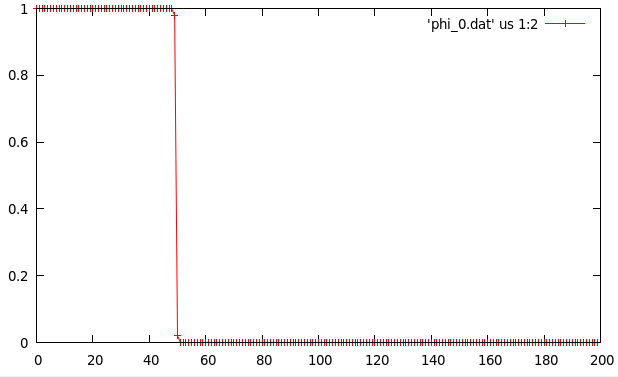
\includegraphics[width=.25\textwidth]{phi_0.png}
\label{timestep 0}
}
\hspace{.25in}
\subfloat[timestep 50000]{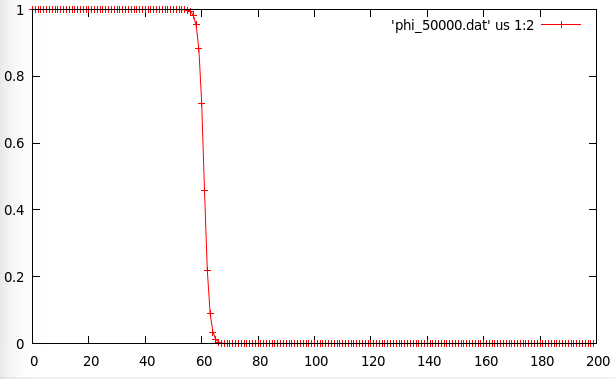
\includegraphics[width=.25\textwidth]{phi_50000.png}
\label{timestep 50000}
}
\hspace{.25in}
\subfloat[timestep 150000]{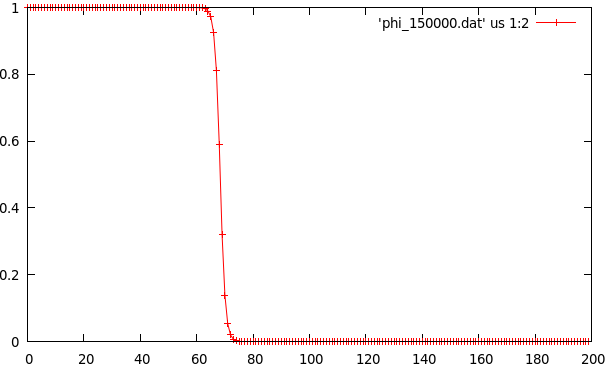
\includegraphics[width=.25\textwidth]{phi_150000.png}
\label{timestep 150000}
}
\centering
\caption{time evolution of the phase field variable $\phi$}
%\label{micros_3}
\end{figure}
 
\begin{figure}[!htbp]
\centering
\subfloat[timestep 0]{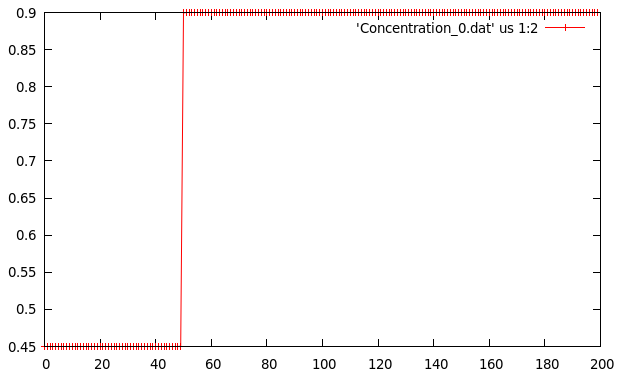
\includegraphics[width=.25\textwidth]{conc_0.png}
\label{timestep 0}
}
\hspace{.25in}
\subfloat[timestep 50000]{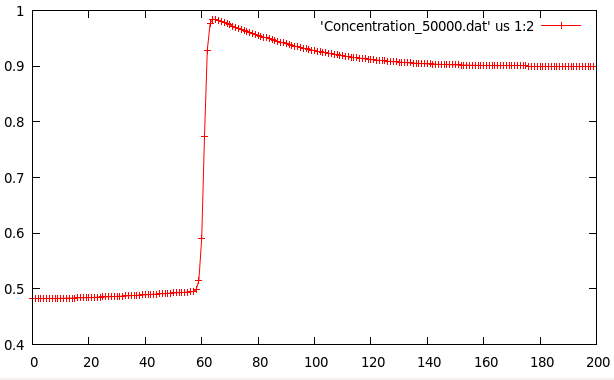
\includegraphics[width=.25\textwidth]{conc_50000.png}
\label{timestep 50000}
}
\hspace{.25in}
\subfloat[timestep 150000]{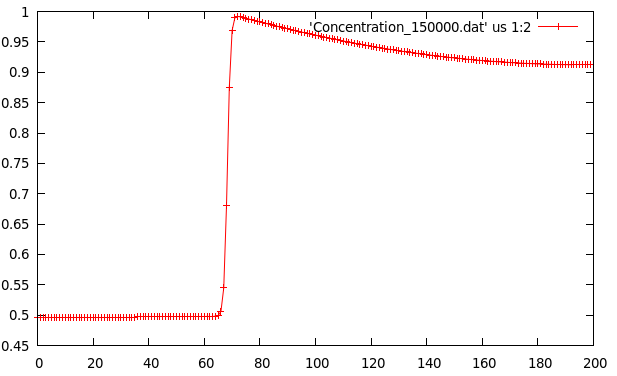
\includegraphics[width=.25\textwidth]{conc_150000.png}
\label{timestep 150000}
}
\centering
\caption{time evolution of concentration}
%\label{micros_3}
\end{figure}

\begin{figure}[!htbp]
\centering
\subfloat[timestep 0]{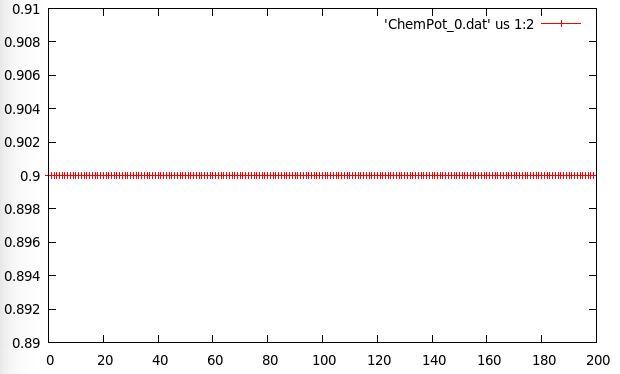
\includegraphics[width=.25\textwidth]{chem_0.png}
\label{timestep 0}
}
\hspace{.25in}
\subfloat[timestep 50000]{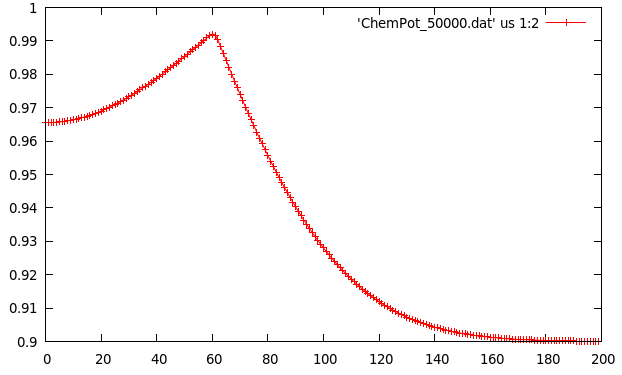
\includegraphics[width=.25\textwidth]{chem_50000.png}
\label{timestep 50000}
}
\hspace{.25in}
\subfloat[timestep 150000]{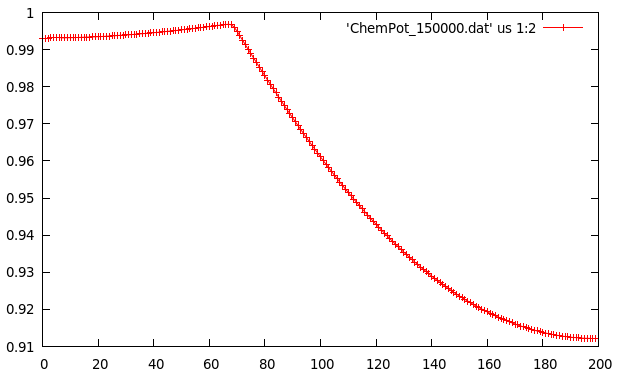
\includegraphics[width=.25\textwidth]{chem_150000.png}
\label{timestep 150000}
}
\centering
\caption{time evolution of chemical potential $\mu$}
%\label{micros_3}
\end{figure}
\newpage

\section{Isotropic Solidification in 2D - only diffusion}

In two dimensions, $\phi$ and $\mu$ fields we represented by two $200\times 200$ meshes. The time update is through forward difference by 
calcualting the partial derivatives of $\phi$ and $\mu$ at each node point. Also, fluid is neglected such that diffusion is the only mode 
transport.\\
$
\tau\epsilon\dfrac{\partial\phi}{\partial t} = \gamma\nabla^{2}\phi -\dfrac{\gamma}{\epsilon}18\phi(1-\phi)(1-2\phi)
					+(k - 1)\mu\left(\mu-\mu_{eq}\right)(6\phi)\left(1-\phi\right)\\
\chi \dfrac{\partial \mu}{\partial t} =  M\nabla^2\mu 
	- 6\left(k-1\right)\mu\phi\left(1-\phi\right)\dfrac{\partial\phi}{\partial t}\\
\nabla^{2}\phi = \dfrac{\phi_{i+1,j}+\phi_{i-1,j}+\phi_{i,j+1}+\phi_{i,j-1} - 4\phi_{i,j}}{(\Delta t)^2}\\
\nabla^{2}\mu = \dfrac{\mu_{i+1,j}+\mu_{i-1,j}+\mu_{i,j+1}+\mu_{i,j-1} - 4\mu_{i,j}}{(\Delta t)^2}	
$
\\

\subsection*{Gibbs Thompson Effect}

Our functional has the form of\\
\\
${\cal F} = \int_{-\infty}^{\infty}(\gamma \epsilon|\nabla\phi|^2 + \dfrac{\gamma}{\epsilon}9\phi^2(1-\phi)^2 + ...)dx$\\
By the equipartition of energy, we have for one dimension,\\

$\gamma\epsilon\left(\dfrac{\partial\phi}{\partial x}\right)^2 = \dfrac{\gamma}{\epsilon}9\phi^2(1-\phi)^2\\
\Rightarrow \dfrac{\partial\phi}{\partial x} = \dfrac{3}{\epsilon}\phi(1-\phi)$\\

Also, we know that total surface energy $\sigma$ is given by the interfacing the interfacial 
energy term over the entire domain,\\
$\sigma = \int_{-\infty}^{\infty}2\gamma\epsilon\left(\dfrac{\partial\phi}{\partial x}\right)^2\cdot dx\\
= \int_{0}^{1}2\gamma\epsilon\left(\dfrac{\partial\phi}{\partial x}\right)\cdot d\phi\\
= 6\gamma\int_{0}^{1}2\phi(1-\phi) d\phi\\
= 6\gamma \left[\dfrac{\phi^2}{2} - \dfrac{\phi^3}{6}\right]_{0}^{1}\\
\Rightarrow \sigma = \gamma\\
$

We also know that at critical radius, surface energy equals the driving force for solidification- 
due to deviation of deviation from equilibrium of the Free energy,
 \\ 
$\dfrac{\sigma}{r} = (k-1)\mu\left(\mu-\mu_eq\right)$ \\
Thus, for a given radius we can calculate a critical $\mu_c$ for which the nuclei is 
stable. For $\mu > \mu_c$ nuclei should grow, otherwise the nuclei should shrink.
 
We used the above relation to calculate the critical $\mu_c$ for a 
radius of 50 units and found out that this Gibbs Thompson relation indeed holds for 
the present model.

\begin{figure}[!htbp]
\centering
\subfloat[timestep 0]{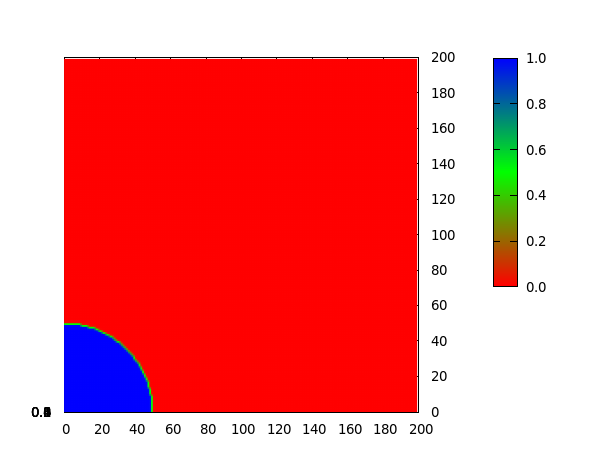
\includegraphics[width=.25\textwidth]{gt_0.png}
\label{timestep 0}
}
\hspace{.25in}
\subfloat[timestep 50000]{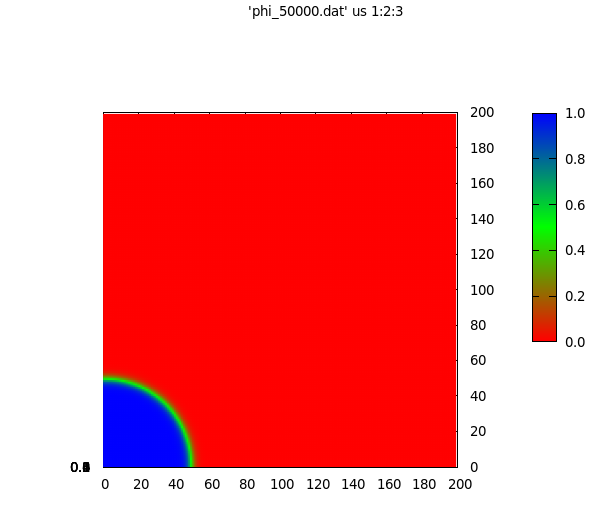
\includegraphics[width=.25\textwidth]{gt_50.png}
\label{timestep 50000}
}
\hspace{.25in}
\subfloat[timestep 150000]{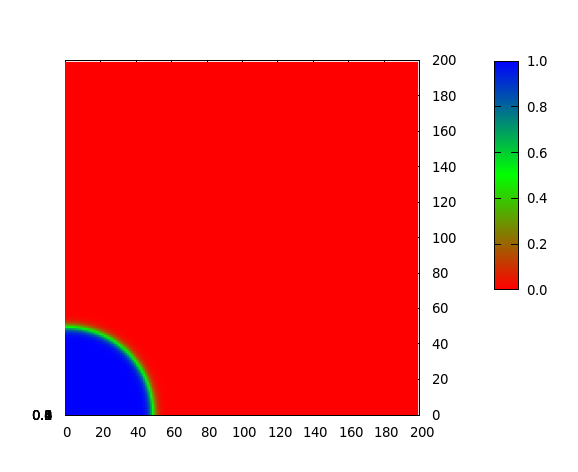
\includegraphics[width=.25\textwidth]{gt_99.png}
\label{timestep 99000}
}
\centering
\caption{Nuclei at critical radius - not growing}
%\label{micros_3}
\end{figure}

\begin{figure}[!htbp]
\centering
\subfloat[timestep 0]{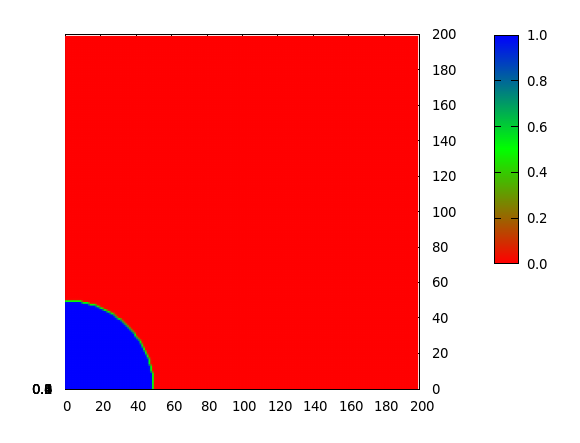
\includegraphics[width=.25\textwidth]{shrink_0.png}
\label{timestep 0}
}
\hspace{.25in}
\subfloat[timestep 50000]{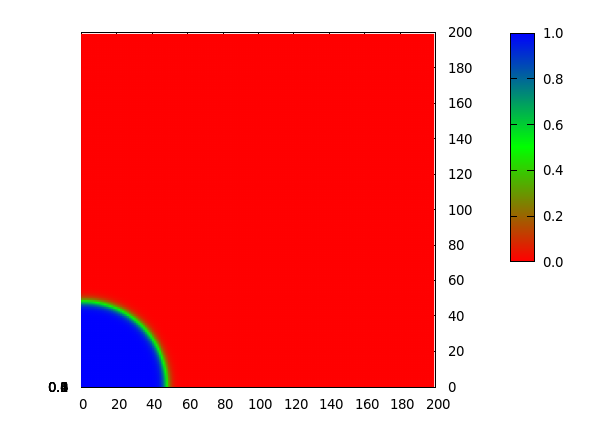
\includegraphics[width=.25\textwidth]{shrink_50.png}
\label{timestep 50000}
}
\hspace{.25in}
\subfloat[timestep 150000]{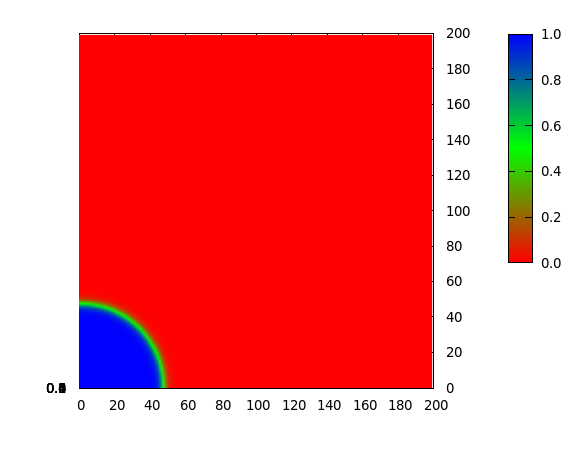
\includegraphics[width=.25\textwidth]{shrink_99.png}
\label{timestep 99000}
}
\centering
\caption{Nuclei Shrinking - $\mu$ less than critical}
%\label{micros_3}
\end{figure}

\begin{figure}[!htbp]
\centering
\subfloat[timestep 0]{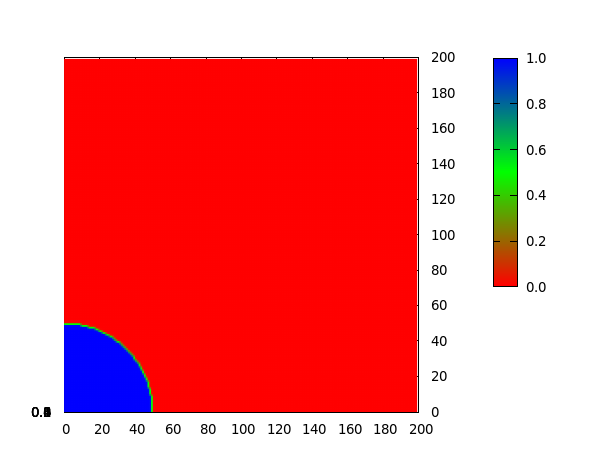
\includegraphics[width=.25\textwidth]{gt_0.png}
\label{timestep 0}
}
\hspace{.25in}
\subfloat[timestep 50000]{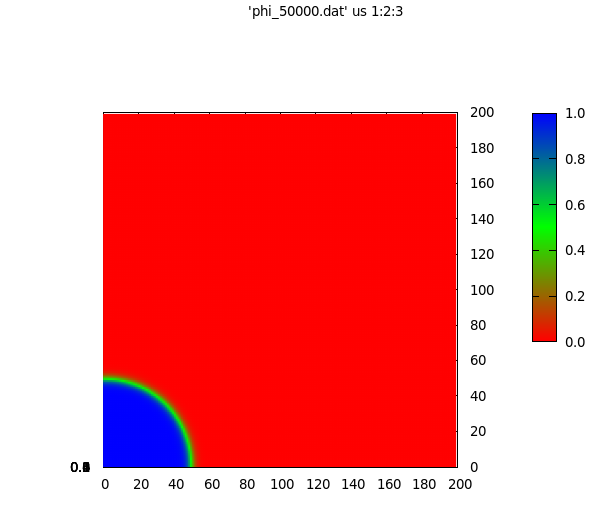
\includegraphics[width=.25\textwidth]{gt_50.png}
\label{timestep 50000}
}
\hspace{.25in}
\subfloat[timestep 99000]{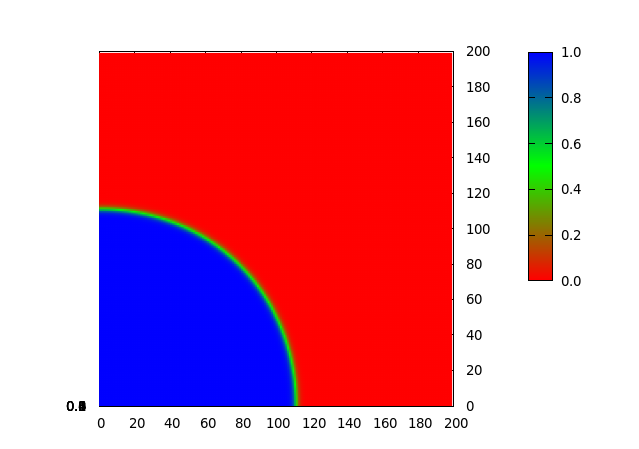
\includegraphics[width=.25\textwidth]{grow_99.png}
\label{timestep 99000}
}
\centering
\caption{Nuclei growing - $\mu$ greater than critical}
%\label{micros_3}
\end{figure}
\newpage
\section{Dendritic Solidification}

\begin{figure}[!htbp]
\centering
\subfloat[timestep 0]{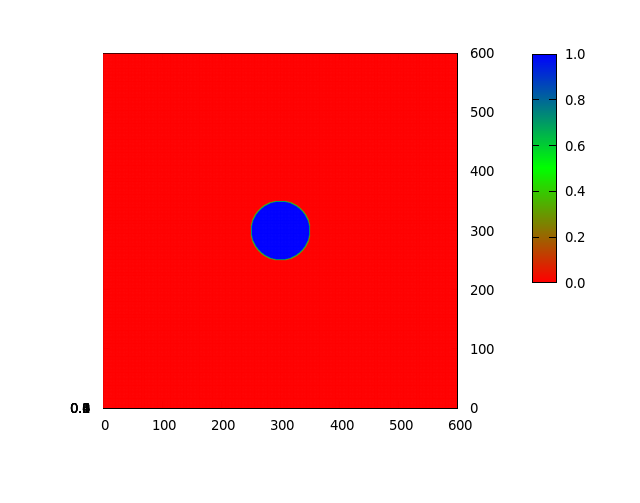
\includegraphics[width=.25\textwidth]{dendrite_0.png}
\label{timestep 0}
}
\hspace{.25in}
\subfloat[timestep 15000]{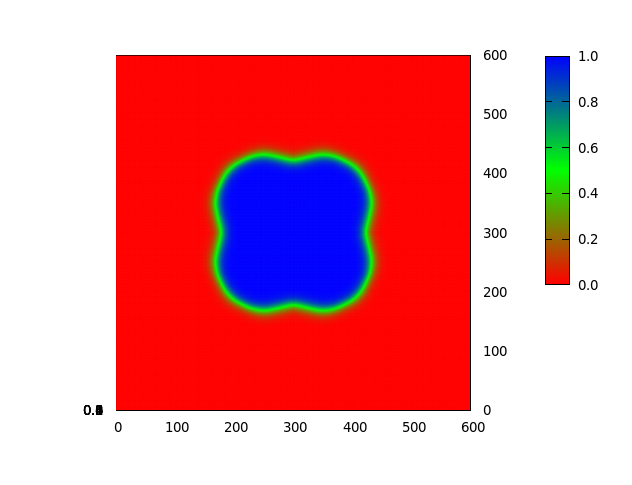
\includegraphics[width=.25\textwidth]{dendrite_15000.png}
\label{timestep 50000}
}
\hspace{.25in}
\subfloat[timestep 30000]{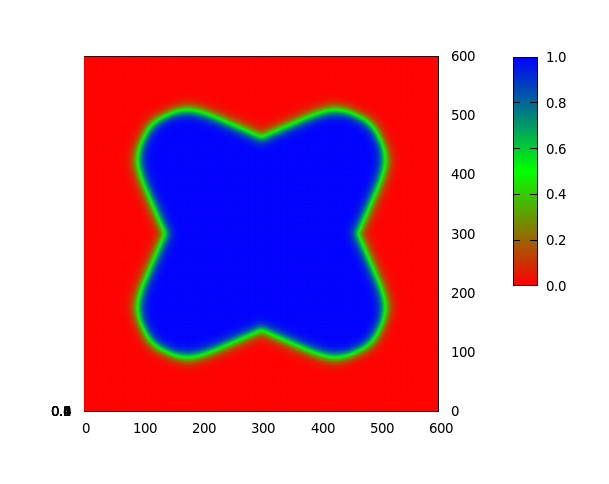
\includegraphics[width=.25\textwidth]{dendrite_30000.png}
\label{timestep 99000}
}
\centering
\caption{Dendritic solidification on introducing anisotropy}
%\label{micros_3}
\end{figure}

\section{Simulating fluid flow in closed space}

\subsection*{Lid Driven Cavity Flow}

\begin{figure}[!htbp]
\centering
\subfloat[timestep 0]{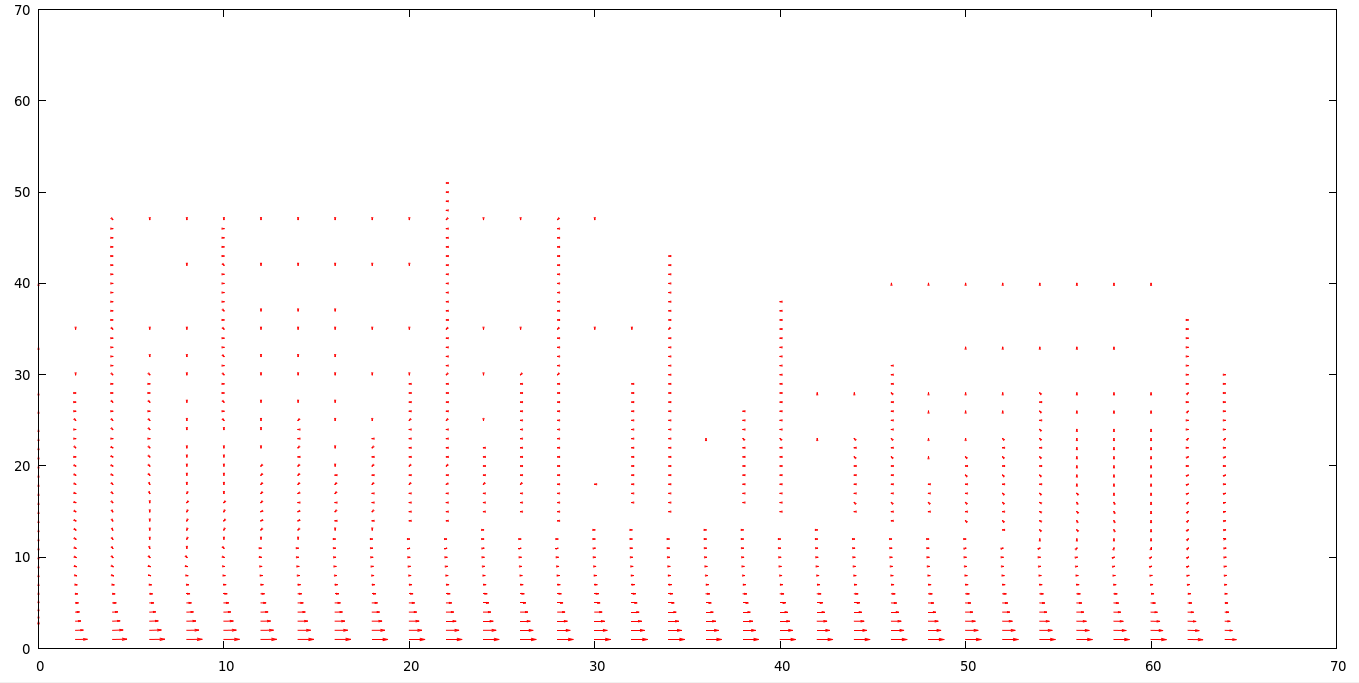
\includegraphics[width=.25\textwidth]{LD_0.png}
%\label{timestep 0}
}
\hspace{.25in}
\subfloat[timestep 10000]{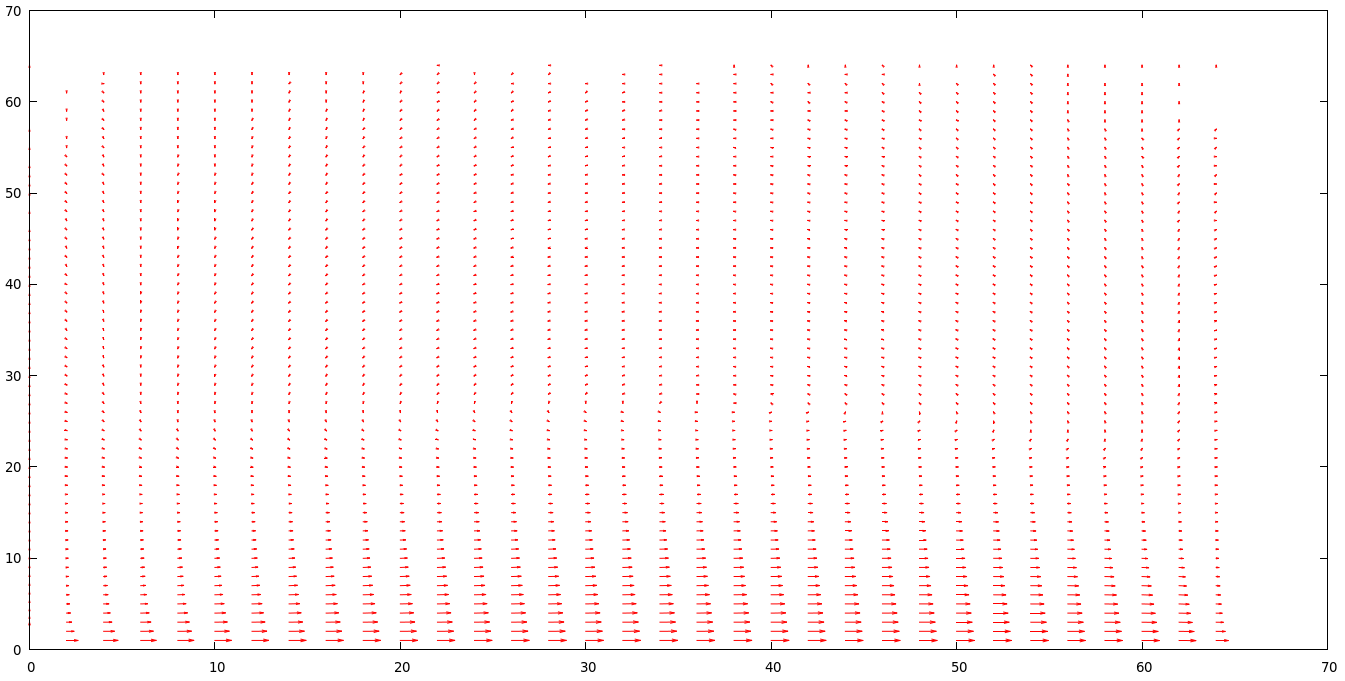
\includegraphics[width=.25\textwidth]{LD_10000.png}
%\label{timestep 10000}
}
\centering
\caption{Lid Driven Cavity Flow; South wall moving left}
%\label{micros_3}
\end{figure}
\subsection*{Poiseuille flow}

\begin{figure}[!htbp]
\centering
\subfloat[timestep 1000]{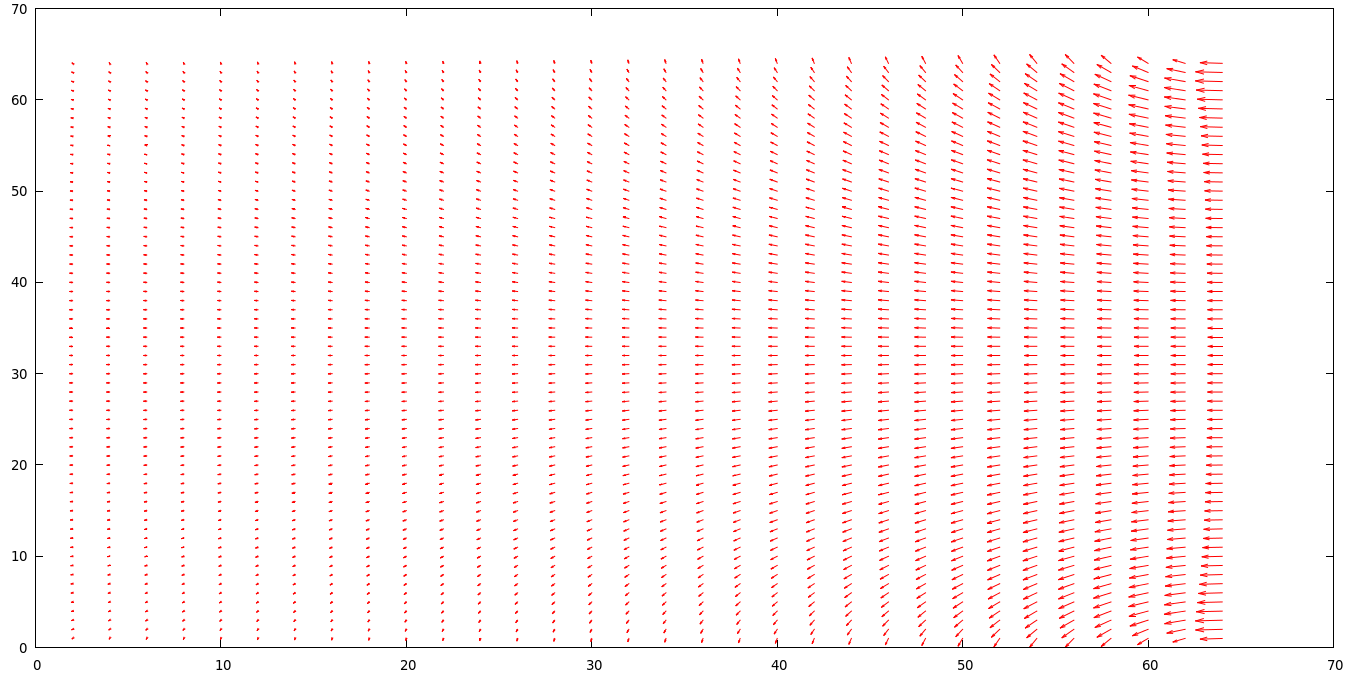
\includegraphics[width=.25\textwidth]{pflow_1000.png}
%\label{timestep 0}
}
\hspace{.25in}
\subfloat[timestep 10000]{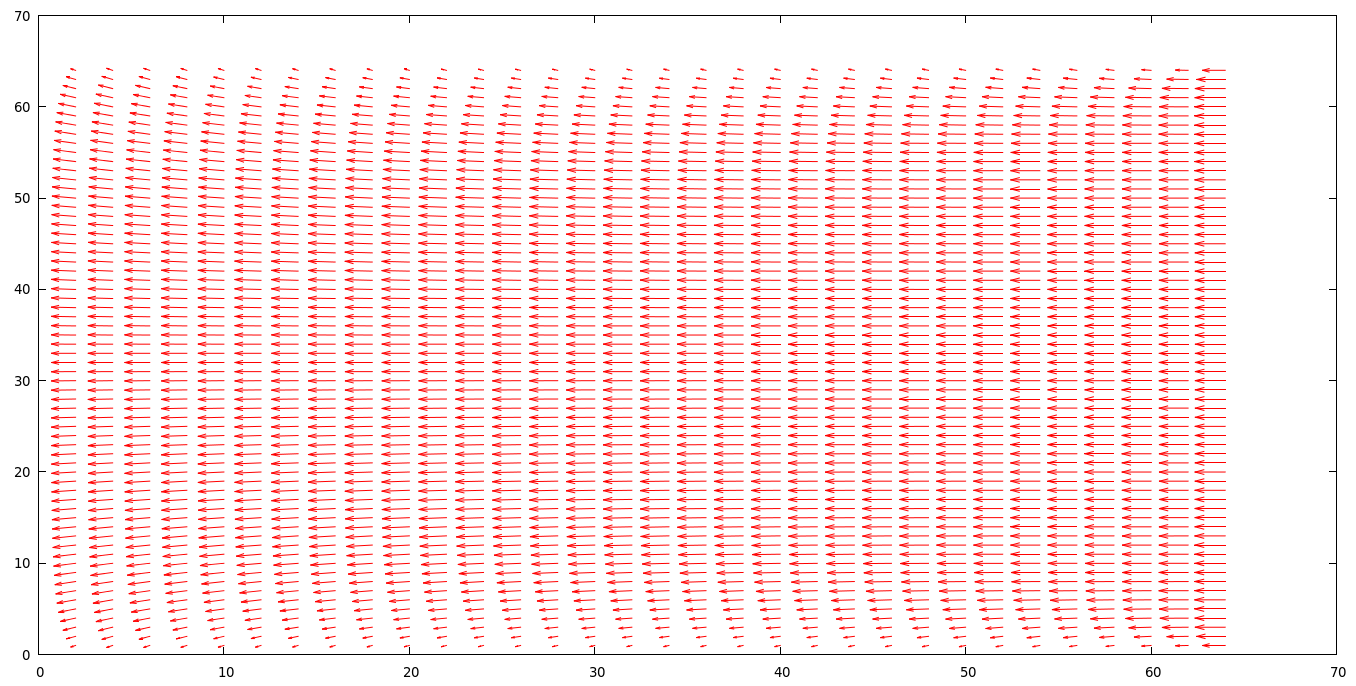
\includegraphics[width=.25\textwidth]{pflow_10000.png}
%\label{timestep 50000}
}
\hspace{.25in}
\subfloat[timestep 50000]{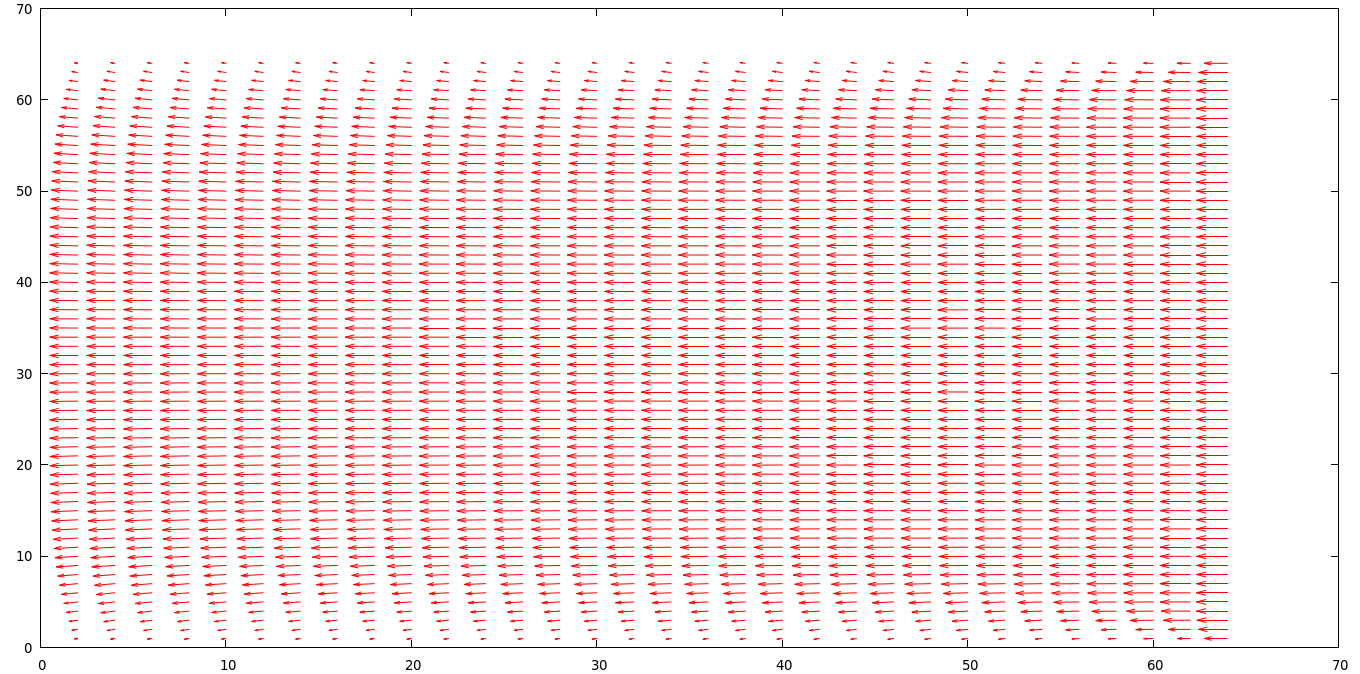
\includegraphics[width=.25\textwidth]{pflow_50000.png}
%\label{timestep 50000}
}
\centering
\caption{Pressure difference between East and West walls}
\end{figure}

\subsection*{Flow around a solid object in a closed space}

\begin{figure}[!htbp]
\centering
\subfloat[timestep 1000]{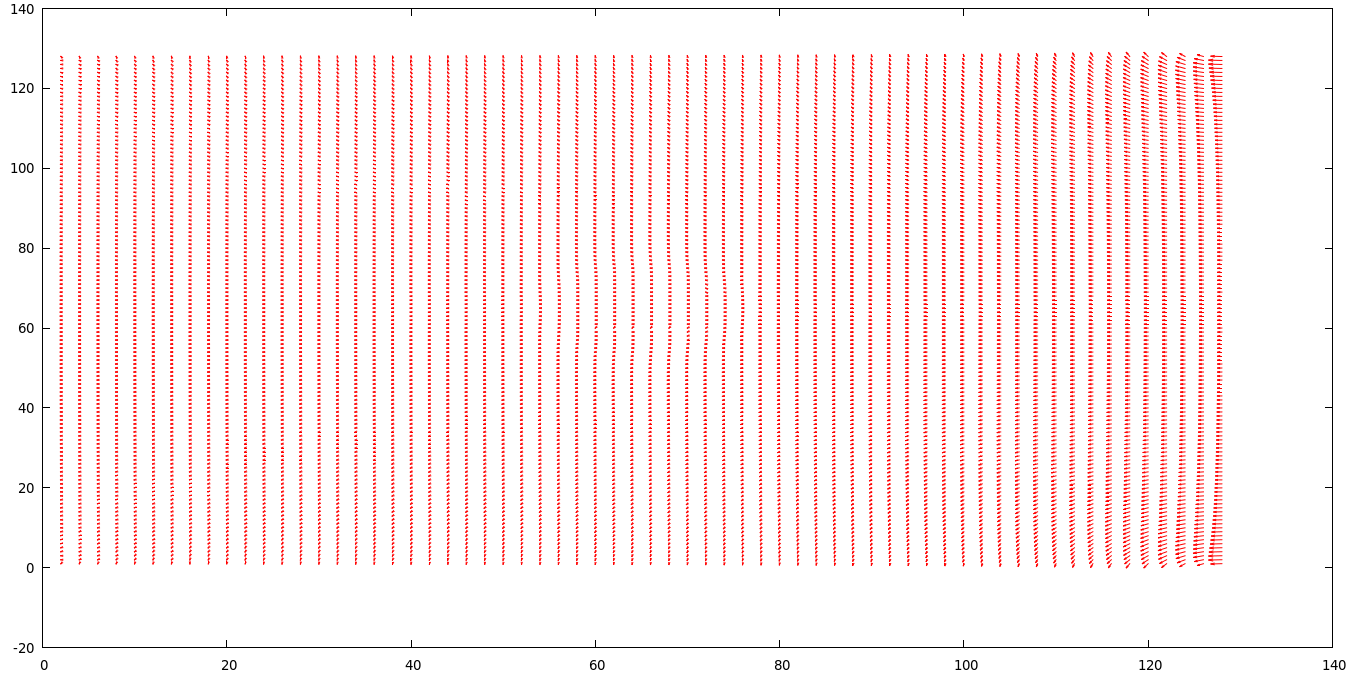
\includegraphics[width=.25\textwidth]{object_1000.png}
%\label{timestep 0}
}
\hspace{.25in}
\subfloat[timestep 10000]{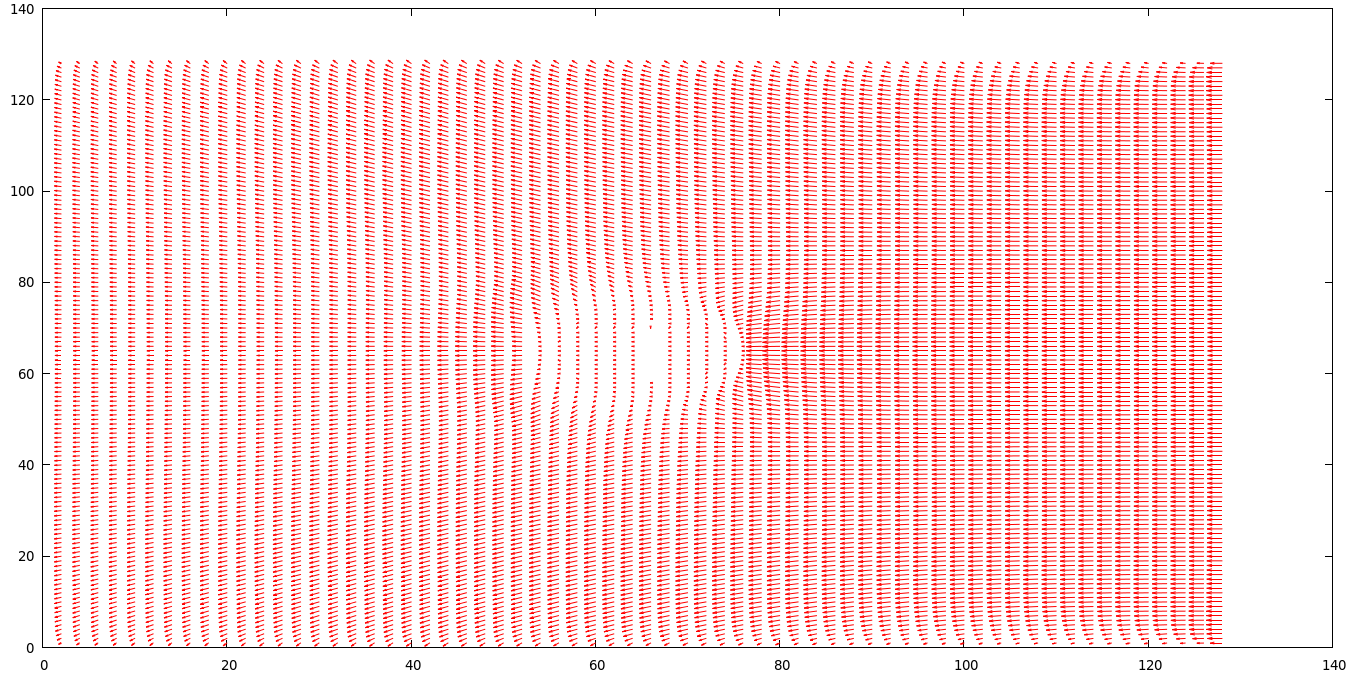
\includegraphics[width=.25\textwidth]{object_10000.png}
%\label{timestep 50000}
}
\hspace{.25in}
\subfloat[timestep 50000]{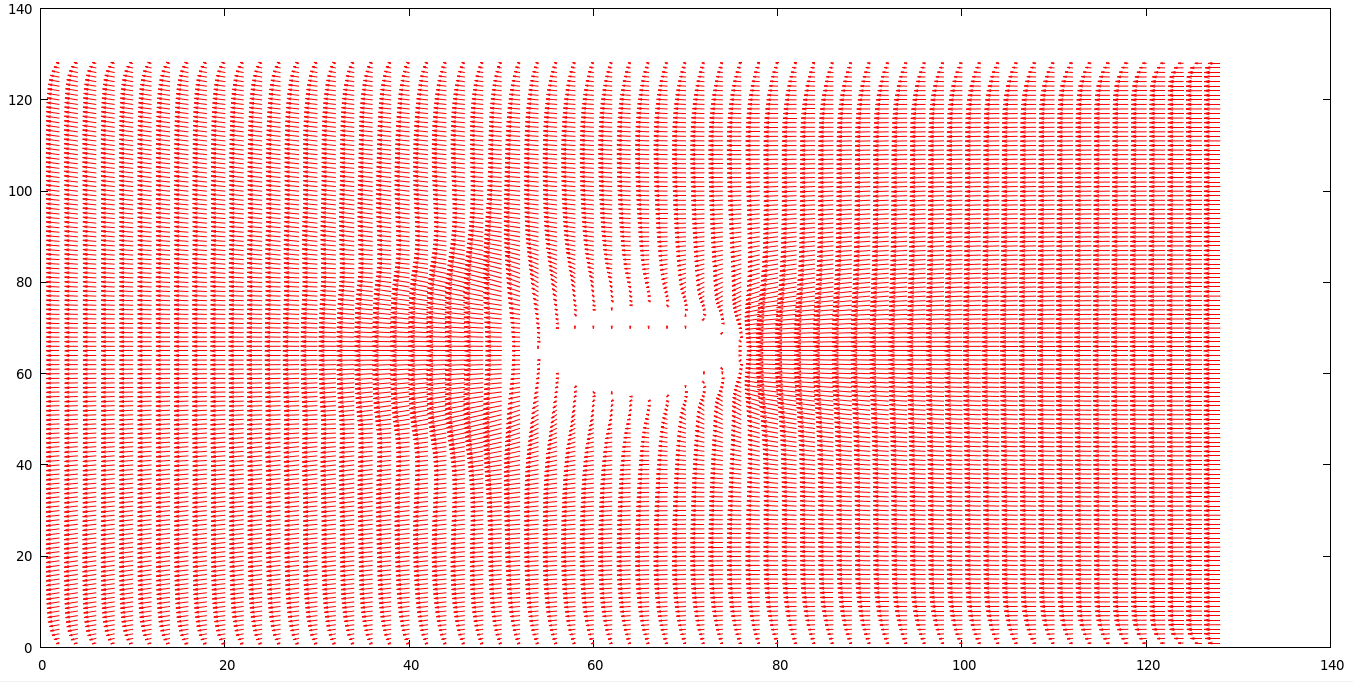
\includegraphics[width=.25\textwidth]{object_50000.png}
%\label{timestep 50000}
}
\centering
\caption{Flow around a solid with a diffuse interface}
\end{figure}

\chapter{Discretisation}

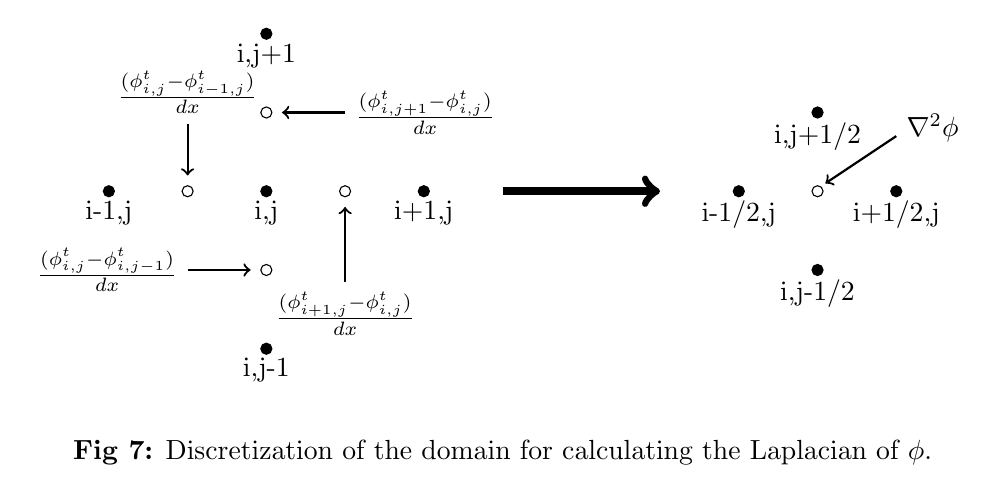
\begin{tikzpicture}
	\filldraw[black] (0,0) circle (2pt)
		node[below] {i,j};
	\filldraw[black] (2,0) circle (2pt)
		node[below] {i+1,j};
	\filldraw[black] (-2,0) circle (2pt)
		node[below] {i-1,j};
	\filldraw[black] (0,2) circle (2pt)
		node[below] {i,j+1};
	\filldraw[black] (0,-2) circle (2pt)
		node[below] {i,j-1};
	\draw[black] (1,0) circle (2pt);
	\draw[black,thick,<-] (1,-0.2) -- (1,-1.15)
		node[below] {$\frac {(\phi_{i+1,j}^t - \phi_{i,j}^t)}{dx}$};
	\draw[black] (-1,0) circle (2pt);
	\draw[black,thick,<-] (-1,0.2) -- (-1, 0.85)
		node[above] {$\frac {(\phi_{i,j}^t - \phi_{i-1,j}^t)}{dx}$};
	\draw[black] (0,1) circle (2pt);
	\draw[black,thick,<-] (0.2,1) -- (1,1)
		node[right] {$\frac {(\phi_{i,j+1}^t - \phi_{i,j}^t)}{dx}$};
	\draw[black] (0,-1) circle (2pt);
	\draw[black,thick,<-] (-0.2,-1) -- (-1,-1)
		node[left] {$\frac {(\phi_{i,j}^t - \phi_{i,j-1}^t)}{dx}$};
	\draw[black,thick,line width=1mm,<-] (5,0) -- (3,0)
		node[below=3 cm] {\textbf{Fig 7:} Discretization of the domain for calculating the Laplacian of $\phi$.};
	\filldraw[black] (8,0) circle (2pt)
		node[below] {i+1/2,j};
	\filldraw[black] (6,0) circle (2pt)
		node[below] {i-1/2,j};
	\filldraw[black] (7,1) circle (2pt)
		node[below] {i,j+1/2};
	\filldraw[black] (7,-1) circle (2pt)
		node[below] {i,j-1/2};
	\draw[black] (7,0) circle (2pt);
	\draw[black,thick,<-] (7.1,0.1) -- (8,0.7)
		node[above=0.1cm,right] {$\nabla^2 \phi$};
\end{tikzpicture}
\\
\begin{tikzpicture}
%\draw (0,0) -- (4,0);
\end{tikzpicture}

\begin{thebibliography}{1}
	
  \bibitem{MS_theory} J.S. Langer, in Chance and Matter edited by J. Souletie, J. Vannenimus 
	and R Stora (North Holland, Amsterdam 1987), p. 629; D Kessler, J Koplik and H Levine, Adv. 
	Phys. 37, 255 (1988); E .A. Brenner and V.I. Mel'nikov, \textit{ibid}. 40, 53 (1991)
	
  \bibitem{langer} J. S. Langer, Phys. Rev. Lett., Volume 44, Number 15, 14 April 1980 

  \bibitem{Stein} I. Steinbach, Acta Materialia 57 (2009) 2640 - 2645

  \bibitem{Tong} Tong et al., Phys. Rev. E, vol. 61, No. 1, January 2000

  \bibitem{Abhik_1} Abhik Chaudhary and Britta Nestler, Phys. Rev. E 85,021602 (2012)
  
  \bibitem{Abhik_2} Britta Nestler and Abhik Chaudhary, Current Opinion in solid State 
  and Materials Science 15(2011) 93-105
  
  \bibitem{Beck} C. Beckermann et al., Jour. of Comp. Phys. 154, 468-496 (1999)
  
  \bibitem{Boet} W.J. Boettinger el al., Annu. Rev. Mater. Res. 2002. 32:163-94

\end{thebibliography}
\end{document}

%\begin{tcolorbox}
%
%blablabla
%
%\begin{align}
%E &= mc^2 & \text{Formula of the universe}
%\end{align}
%\lipsum[1]
%\lipsum[2]
%\lipsum[1]
%\lipsum[2]
%\lipsum[3]
%\lipsum[2]
%Hoaray
%
%\end{tcolorbox}

%\begin{mdframed}
%\lipsum[1]
%\begin{equation}
% f(x) = \sin(x)
%\end{equation}
%\lipsum[2]
%\end{mdframed}